\chapter{Metodo}
\label{ch:teoria}

Nel seguente capitolo vengono proposti gli aspetti teorici utili nella comprensione del modello, degli strumenti utilizzati e delle condizioni imposte dalla simulazione sulla natura del sistema.

\section{Espansione di Lie-Trotter}
\label{sec:LT}

Per espandere l'operatore, si è scelto di utilizzare un risultato noto con il nome di "Formula di Lie-Trotter":
\begin{equation}
    \centering
     \exp \left({A} + {B}\right) = \lim_{n\to\infty } \left[  \exp \left(\frac{A}{n}\right)  \exp \left(\frac{B}{n}\right) \right] ^{n} \; \text{,}
    \label{eq:LT_formula}
\end{equation}
dove $A$ e $B$ rappresentano due generici operatori lineari non commutanti.
Dall'eq. (\ref{eq:LT_formula}) si può dimostrare che vale la seguente espansione 
\begin{equation}
    \centering
    %\exp \left(\tau ({A} + {B})\right) 
    e^{\tau ({A} + {B})}
    = \prod _{j=1} ^{n}  \exp \left( \tau A c_{j}\right)   \exp \left(\tau B d_{j}\right) + O(\tau^{n}) \; \text{,}
    \label{eq:LT_expantion}
\end{equation}
con $c_{i}$ e $d_{i}$ coefficienti reali.

All'interno del software sono stati implementai tre diversi livelli di profondità, troncando la produttoria al primo ordine
\begin{equation}
    \centering
    %\exp \left(\tau ({A} + {B})\right)
    e^{\tau ({A} + {B})} 
    =  \exp \left( \tau A \right)   \exp \left(\tau B \right) + O(\tau) \; \text{,}
    \label{eq:LT_1}
\end{equation}
al secondo ordine 
\begin{equation}
    \centering
    %\exp \left(\tau ({A} + {B})\right) 
    e^{\tau ({A} + {B})}
    =  \exp \left(\frac{1}{2} \tau A \right)   \exp \left(\tau B \right)   \exp \left(\frac{1}{2} \tau A \right) +  O(\tau^{2}) \; \text{,}
    \label{eq:LT_2}
\end{equation}
e al terzo ordine

\begin{multline}
    %\exp \left(\tau ({A} + {B})\right) 
    e^{\tau ({A} + {B})}
    =  \exp \left( \tau A \right)   \exp \left( - \frac{1}{24}  \tau B \right)  \exp \left( - \frac{2}{3} \tau A \right)   \\    \exp \left( \frac{3}{4} \tau B \right)  \exp \left( \frac{2}{3} \tau A \right)   \exp \left( \frac{7}{24} \tau B \right)   +  O(\tau^{3}) \; \text{.}
    \label{eq:LT_3}
\end{multline}

%Sistema...
Per fissare i coefficienti $c_{i}$ e $d_{i}$ è necessario uguagliare l'espansione in serie di potenze con l'espansione di Lie-Trotter, troncate allo stesso ordine, in modo che termini uguali abbiano lo stesso peso.
Al fine di confermare l'eq. (\ref{eq:LT_expantion}) e esplicitare il processo seguito, si riporta il calcolo nel caso $n=1$.
\begin{equation}
    \begin{split}
        %\exp \left(\tau ({A} + {B})\right) 
        e^{\tau ({A} + {B})}
        & = I + \tau(A + B) + \frac{\tau^{2}}{2} (A + B)^2 + O(\tau^{3})  \\
        & = I + \tau(A + B) + \frac{\tau^{2}}{2} (A^2 + AB + BA + B^2) + O(\tau^{3}) \; \text{,}
    \end{split}
    \label{eq:std_expantion}
\end{equation}
\begin{equation}
    \begin{split}
        %\exp \left(\tau A c_{1} \right)  \exp \left(\tau B d_{1} \right) 
        e^{\tau A c_{1}} \, e^{\tau B d_{1}} 
        & = \left[ I + \tau A c_{1}  + \frac{\tau^{2}}{2} A^2 c_{1}^2 + O(\tau^{3}) \right] \left[  I + \tau B d_{1} + \frac{\tau^{2}}{2} B^2 d_{1}^2+ O(\tau^{3}) \right] \\
        & = I + \tau (A c_{1} + B d_{1} ) + \frac{\tau^{2}}{2} (A^2 c_{1}^2 + 2  A B c_{1}d_{1} + B^2 d_{1}^2) + O(\tau^{3}) \; \text{.}
    \end{split}
    \label{eq:first_proof}
\end{equation}
Come si può vedere dal confronto tra l'eq. (\ref{eq:std_expantion}) e l'eq. (\ref{eq:first_proof}), è obbligatoria la scelta $c_{1} = 1$ e $d_{1} = 1$ per ottenere l'uguaglianza al primo ordine.
Dalla differenza tra le due si ottiene che 
\begin{equation}
         \exp \left(\tau A\right)  \exp \left(\tau B\right) =  \exp \left(\tau ({A} + {B}) + \frac{\tau^{2}}{2} [A, B] + O(\tau^{3})\right) \; \text{,}
    \label{eq:proof}
\end{equation}
in linea con l'eq. (\ref{eq:LT_expantion}). Ad ordini superiori la complessità aumenta molto rapidamente, per trovare i coefficienti è, infatti, necessario risolvere un sistema non lineare di $\sum_{i=1}^{n} 2^{i} $ equazioni in $2n$ incognite. Un tale sistema risulterà quasi sempre inderterminato, permettendo ampia scelta tra soluzioni possibili. Al fine di ridurre il numero di operazioni, la scelta da operare dovrebbe in primo luogo azzerare il numero più alto di coefficienti in modo da rendere banali i termini esponenziali %\footnote{ $ \; e^0 = 1$}.
e inoltre predilegere quelle scelte per cui si ottengono coefficienti uguali.
Ad esempio, al secondo ordine si ottiene come soluzione
\begin{equation}
    c_{1} = 1 + \frac{1}{2 + d_{2} -1}  \; \text{,} \qquad  d_{1} = 1 -d  \; \text{,} \qquad c_{2} = - \frac{1}{2(d_{2}-1)}  \; \text{,} 
    \label{eq:2_order_sol}
\end{equation}
per cui per $d_2 = 0$ si semplifica l'ultimo termine.
\begin{equation}
    c_{1} = \frac{1}{2} \; \text{,}  \qquad 
    d_{1} = 1 \; \text{,}  \qquad
    c_{2} = \frac{1}{2}  \; \text{.}
\end{equation}
Sfortunatamente non è possibile azzerare nessun coefficiente al terzo al ordine.
Non esiste un metodo che sia univocamente riconosciuto come migliore rispetto ad altri per trovare i coefficienti ad ordini superiori. Il problema però è stato affrontato da diversi autori in letteratura, perciò è possibile fare uso dei loro risulatati. Tra i metodi più utilizzati e di maggior successo, per n pari, si vuole ricordare il metodo frattale \textcolor{red}{citazione}.

Il motivo della scelta di usare un'espansione del tipo in eq. (\ref{eq:LT_expantion}) al posto di un'espansione del tipo 
\begin{equation}
         \exp \left(\tau ({A} + {B})\right) = I + \tau(A + B) + \frac{\tau^{2}}{2} (A + B)^2 + \frac{\tau^{3}}{3!} (A + B)^3 + O(\tau^{4})  \; \text{,} 
    \label{eq:std}
\end{equation}
risiede in una fondamentale proprietà dell'eq. (\ref{eq:LT_expantion}), tale espansione infatti conserva la natura unitaria dell'operatore di evoluzione, ciò non accade utilizzando l'eq. (\ref{eq:std})\cite{Hatano:exp}.
L'operatore di evoluzione in eq. (\ref{eq:U_inf}) ha la forma di un esponenziale complesso, quindi approssimato tramite l'eq. (\ref{eq:LT_expantion}) 
\begin{equation}
    \centering
     \exp \left(\frac{-i \, \delta t }{\hbar}  \, (\hat{V} + \hat{T})\right)   = \prod _{j=1} ^{n}  \exp \left(\frac{-i \, \delta t }{\hbar} \, \hat{V} \, c_{j}\right)   \exp \left(\frac{-i \, \delta t }{\hbar} \, \hat{T} \, d_{j}\right) + O(\tau^{n}) \; \text{,}
    \label{eq:sim_exp}
\end{equation}
diviene un prodotto di esponenziali complessi sempre unitario.

\section{Soluzione numerica} %{Discretizzazione dello spazio e applicazione dell'operatore $\hat{U}$ }
\label{sec:disc}

Per risolvere numericamente è necessario definire uno spazio $x$ finito e discreto di punti ${x_i}$ dove campionare la funzione d'onda. In un tale spazio è possibile applicare un numero arbitrario di volte un operatore approssimato del tipo in eq. (\ref{eq:sim_exp}) ad una generica funzione $\psi_{0}(x_i,t_{0})$ e risolvere l'eq. (\ref{eq:Sc_1D}).

Per rendere l'algoritmo più efficiente si utilizza un'ulteriore accortezza. 
%perché si usa la DFT e non si fa la derivata?
Poiché gli algoritmi di differenziazione numerica sono poco efficienti \textcolor{red} {vorrei inserire un commento quantitativo ma non ho trovato referenze in merito} %comportamento asintotico
i termini %$  \exp \left(\nicefrac{-i}{\hbar} \; \delta t \, \hat{T} \, d_{j}\right)$ 
in cui ad esponente compare l'operatore $\hat{T}$ si applicano nella rappresentazione dei momenti. In tale rappresentazione $\hat{p}^2$ si comporta come una semplice moltiplicazione 
\begin{equation}
    \centering
    - \hbar^2 \frac{\partial^{2}}{\partial x^{2}} \longrightarrow p^{2} \; \text{.}
    \label{eq:p^2}
\end{equation}
Per cambiare rappresentazione, come noto, si utilizza la trasformata di Fourier, i cui algoritmi numerici hanno un comportamento asintotico $O(n \log n)$. Alla procedura da eseguire, per ogni passo $\delta t$ e per ogni $n$, nello sviluppo si aggiungono una trasformata e una antitrasformata a seconda del termine che si sta applicando.
\begin{equation}
    \centering
     \exp \left(- \frac{i}{h} \, c_{j} V(x)\right) \mathcal{F}^{-1} \, \left[  \exp \left(- \frac{i}{h} \, d_{j} \, \frac{p^2}{2m} \right) \mathcal{F} \, \left[  \psi(x, t) \right] \right] \; \text{.}
    \label{eq:trasf_anti}
\end{equation}
Poiché si utilizza uno spazio discreto, è necessario definire la trasformata discreta Fourier.

\subsection{Trasformata discreta di Fourier}
\label{sec:DFT}

Si considera lo spazio degli $x$ finito e discreto di $N$ punti $x_{k}$ tale per cui 
\begin{equation}
    \centering
    0 \le x \le L \qquad \text{con} \quad x_{k} = \frac{L}{N}  k \, \text{,} \quad  k = 0, \, \dots\, , \,  N-1 \, \text{.}
    \label{eq:x_space}
\end{equation}
La trasformata discreta di Fourier è definita in analogia con la sua controparte continua
\begin{equation}
    \begin{split}
        \tilde{\psi}(p) & \approx \frac{1}{\sqrt{2 \pi \hbar}} \frac{L}{N} \sum_{k=0}^{N-1}  \exp \left(-i \frac{p}{h} x_{k} \right) \psi(x_{k}) \\
        & = \frac{1}{\sqrt{2 \pi \hbar}} \frac{L}{N} \sum_{k=0}^{N-1}  \exp \left(-i \frac{p}{h} \frac{L}{N} k \right) \psi ( \frac{L}{N} k ) \, \text{.}
    \end{split}
    \label{eq:dft}
\end{equation}
Si noti che, poiché lo spazio degli $x$ è finito, si induce una periodicità in $\tilde{\psi}(p)$ dovuta al termine
\begin{equation}
    \centering
    \exp \left(-i \frac{p}{h} \, \frac{L}{N} \, k \right) \, \text{.}
\end{equation}
Infatti
\begin{equation}
    \centering
    \tilde{\psi}(p) = \tilde{\psi}(p + P) \quad \text{per}  \quad  \exp \left(-i \frac{P}{h} \frac{L}{N} k \right) = 1 \, \text{,}
    \label{eq:p_periodicity}
\end{equation}
questo si ottiene quando $P = 2 \pi \hbar \, N / L  $.
Per questo motivo si definisce la trasformata in modo che sia univoca limitando lo spazio dei $p$
\begin{equation}
    \centering
    0 \le p \le 2 \pi \hbar \frac{N}{L} \qquad \text{con}  \quad p_{j} = \frac{2 \pi \hbar}{L} j \, \text{,} \qquad  j = 0, \, \dots\,,\, N-1 \, \text{.}
    \label{eq:p_space}
\end{equation}
In definitiva si defisce la trasformata
\begin{equation}
    \tilde{\psi}_j = \frac{1}{\sqrt{2 \pi \hbar}} \frac{L}{N} \sum_{k=0}^{N-1}  \exp \left(-i \frac{2 \pi}{N} j k\right) \psi_k \quad \text{con}  \quad \psi_k \equiv \psi \left( \frac{L}{N} \, k \right) \, \text{,}
    \label{eq:dft_final}
\end{equation}
mentre l'antitrasformata
\begin{equation}
    \psi_k = \frac{\sqrt{2 \pi \hbar}}{L} \sum_{j=0}^{N-1}  \exp \left(-i \frac{2 \pi}{N} j k\right) \tilde{\psi_j} \, \text{.}
    \label{eq:dft_anti}
\end{equation}
\begin{figure}
    \centering
    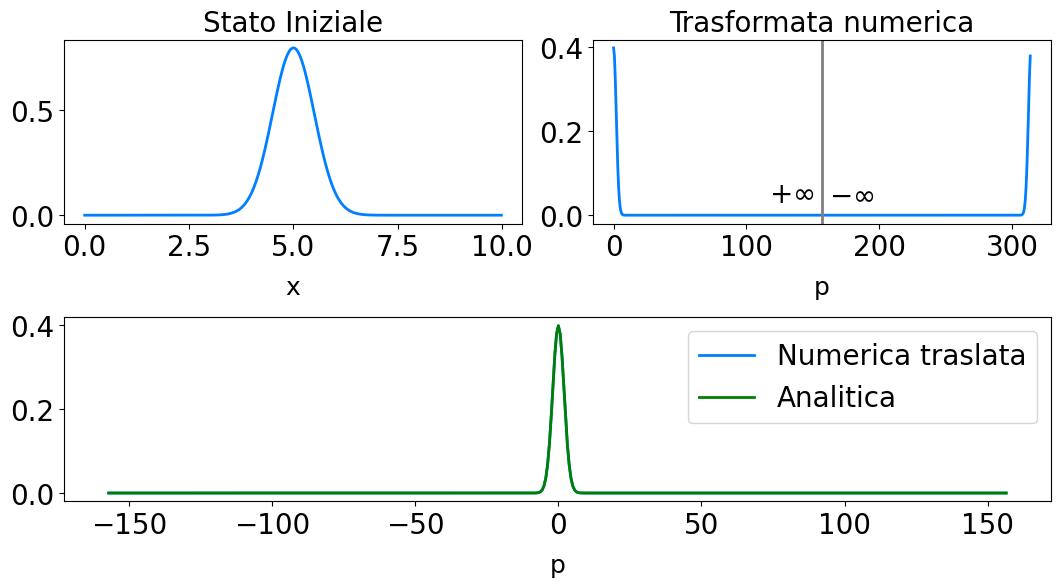
\includegraphics[width = 0.7\textwidth]{immagini/fourier.png}
    \caption{Modulo della trasformata di Fourier di una funzione gaussiana centrata in $x_0 = 5$. Notare come per ottenere la vera rappresentazione fisica nello spazio dei momenti sia necessario eseguire una traslazione rigida della soluzione numerica per $p >   \pi \hbar \, N / L  $}
    \label{fig:dft_shift}
\end{figure}
La discretizzazione dei valori introduce un'altra problematica. La trasformata discreta mappa tutti i valori di $\tilde{\psi}(p)$ in un intervallo che non è simmetrico rispetto all'origine, come fa invece la trasformata continua. Se si considera un periodo $ 0 \le p \le 2 \pi \hbar \, N / L  $ in questo spazio sono mappati tutti i valori di $p$ da $- \infty$ a $+ \infty$, ma sono disposti in ordine inverso. Nella prima metà, tra $ 0 \le p \le \pi \hbar \, N / L  $, sono mappati i valori tra $0$ e $+ \infty$, mentre nella seconda metà tra  $ \pi \hbar \, N / L  < p \le 2 \pi \hbar \, N / L $ sono riportati i valori corrispondenti all'intervallo tra $- \infty$ e $0$. Per costruire, quindi, la vera rappresentazione fisica della funzione d'onda nello spazio dei $p$ è necessario eseguire una traslazione rigida della $\tilde{\psi}(p)$ dall'intervallo $ \pi \hbar N / L < p \le 2 \pi \hbar \, N / L $ all'intervallo $ - \pi \hbar \, N / L  < p \le 0 $, come si può vedere dall'esempio riportato in figura (\ref{fig:dft_shift}).


\section{Conidizioni e vincoli sul sistema} %{Limiti e criticità}
\label{sec:limits}

I principali limiti della simulazione sono dovuti al processo di discretizzazione. 
La discretizzazione dello spazio impone ovvi limiti sulla scelta dei parametri spaziali, poiché essendo lo spazio della simulazione limitato, si perde informazione su qualsiasi oggetto definito al di fuori dell'intervallo $ 0 \le x \le L$. È quindi banale, ma necessario, fare in modo che la funzione d'onda sia interamente definita all'interno dell'intervallo, a meno di porzioni infinitesime. 

La discretizzazione spaziale introduce, inoltre, due criticità dovute alla natura della trasformata discreta di Fourier. In prima istanza bisogna porre particolare attenzione alla scelta dello stato iniziale, poiché non solo è limitato lo spazio diretto, ma lo è anche lo spazio dei momenti. La discretizzazione pone dei limiti non solo sui parametri spaziali della funzione d'onda, ma anche su quei parametri capaci di modificare la forma del profilo nello spazio nei momenti. Nuovamente è necessario che, a meno di infinitesimi, tutta l'informazione nello spazio dei momenti sia contenuta nell'intervallo $ - \pi \hbar \, N / L  < p \le \pi \hbar \, N / L  $. 
Inoltre la periodicità della trasformata di Fourier genera un effetto per cui un per profilo uscente da un estremo dello spazio viene propagata l'evoluzione come entrante dall'altro estremo dello spazio. Tale effetto disturba l'evoluzione della funziona d'onda originale, rendendola scorretta. Scegliendo opportunamente i parametri, è possibile ovviare a questo problema facendo in modo che le conseguenze di questo effetto si manifestino a tempi maggiori di quelli necessari ad ottenere i risultati desiderati. 
\textcolor{red}{ Se, però, si volesse simulare l'andamento di un sistema per tempi lunghi è possibile ovviare a questo problema modificando la forma del potenziale agli estremi dell'intervallo. Se, infatti, si modifica $V$ in maniera tale per cui 
\begin{equation}
    V'(x) = 
        \begin{cases}
            V(x) \quad &\lambda < x < L - \lambda \\ 
             \exp \left(-i \, s\right) &\quad  \text{altrove}
        \end{cases}
    \quad s, \lambda \in \mathbb{R} \, \text{,}
    \label{eq:stp_bound}
\end{equation}
risulterà che la funzione d'onda verrà smorzata esponenzialmente ai bordi. La scelta di $s$ e $\lambda$ deve essere opportunamente valutata in modo da ottenere il risulato desiderato. Per valori di $s$ ed $\lambda$ troppo piccoli lo smorzamento non sarà sufficiente a rendere l'effetto trascurabile. D'altra parte all'aumentare di $s$ aumenta la riflessione dovuta allo smorzamento, altro effetto da voler minimizzare. }

La discretizzazione temporale introduce un valore massimo possibile per il potenziale, dovuto ai termini $ \exp \left(- i V c_{j} \, \delta t\right)$, che sono funzioni periodiche. \textcolor{red}{Dovrei entrare più nel dettaglio?} %più dettagli? Potrei introdurre una parametrizzazione lineare per V e far vdere che per |V| > \frac{2 \pi}{\delta t c_j} rimappo gli stessi valori dell'intervallo 0 \le |V| \le \frac{2 \pi}{\delta t c_j}
Bisogna, quindi, considerare la seguente condizione
\begin{equation}
    \underset{[0, L]}{\max} \; \abs{V(x)} < \frac{2 \pi}{\delta t \, c_{j}} \, \text{.}
    \label{eq:V_max}
\end{equation}
In alcuni casi è possibile ovviare a questa problematica tramite opportune estensioni della funzione d'onda, vedi la sezione \ref{sec:inf}


